
\section{Design}
\begin{figure*}[ht]
    \centering
    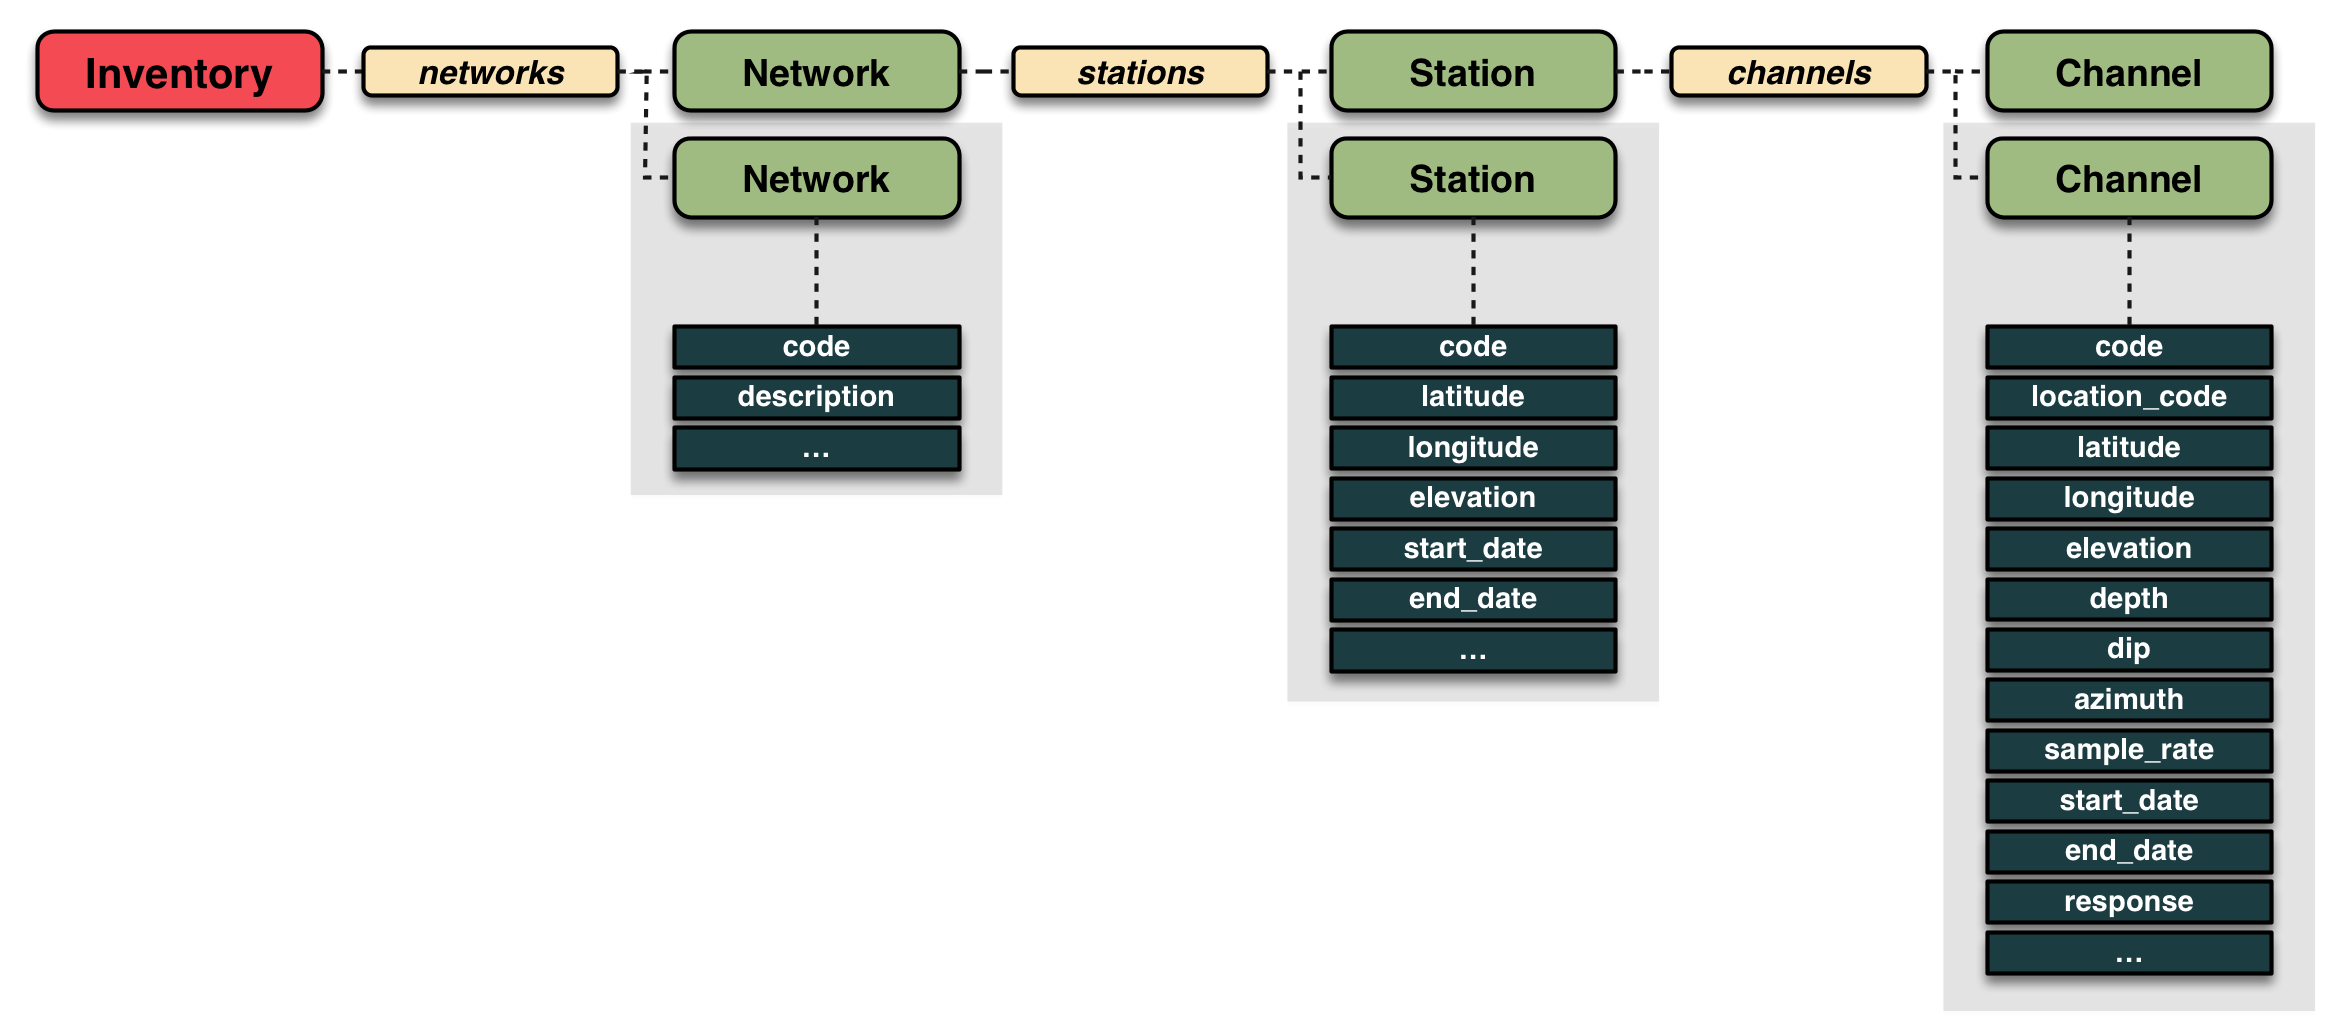
\includegraphics[scale = 0.7]{reportImgs/Inventory.png}
    \caption{A diagram of the obspy data structure, from the documentation}
\end{figure*}



Before being deployed, settings must be set on the devices, which can be done through a smartsolo data transfer rack, and the soloLite software. 
The most important settings on smartsolo devices are their sample rate, and channel gain. 
After its been deployed once a smartsolo has been retrieved from the ground and the dirt cleaned off, it needs to be  positioned in a smartsolo rack transfer socket for its data can be read via usb connection.
The waveforms are stored in collections of 256mb miniseed files, and everything else goes into a file titled DigiSolo.LOG. All the metadata needed for an experiment can be retrieved from this file, 
which holds a great of other useful information. Infact, timestamped data is collected in DigiSolo.LOG for over 95 parameters that cover everything from gps records, booting and device info, 
memory fill, the starting time of each miniseed file, and more, which all gets read to be processed in pythons seismic array package, obspy. 

Obspy has a specific, nested object  structure for describing seismic arrays. At the top of this structure are Inventory objects. 
The inventory objects hold network objects. Network objects hold station objects, representing geophones, and each station has three channel components
to represent the x,y,z components of each geophone.

Rather than manually coding such a large number of details, it is better write a script, which as it reads through the smartsolo log, keeps a dict to track every 
parameter its seen in the file above. It either adds a new entry, when a novel entry parameter is encountered, or  adding to a pre-existing data list. 
The time, if available, is extracted from the rest to be used as an index. This way, everything in the entire log file gets read into python in a clean syntax. 
 Once this is complete, Some of the time series require further processing 
which reduces them to a single metric value. The SmartSolo GPS records values every few minutes, and a simple average is sufficient for 
position and orientation, but it's necessary to run an outlier detection first, because some of the timeseries collect spurious data, even if only during deployment and collection.
Then,  object-oriented inheritence provides a convienent way to tie data directly to the obspy objects. With a class SS\_Station, written in extension of the Obspy station objects,
SS\_Stations have been extended with a readLog function to be called during their initialization. SS\_Net and  SS\_Inventory are similarly defined. 
Functions are then written to SS\_Net that iterate initialization, plotting, and other operations for each station in the network, where necessary.

The smartsolo transfer function, which defines its frequency response, however, can not be accurately deduced from data within the LOG file. Instead, 
Smartsolo has provided a single testing port for such data. The testing port sits aside the data transfer ports, can be operated using SmartSolo's testing software, 
and actually pulses a waveform to each channel for the device, simultaneously recording its response for the devices, and storing the records in an excel sheet.
More scripting is then required for each device to be able to find the test which matches within these files, extract the data, and then apply further mathematical processing to predict 
and define the devices transfer function in way that can be read and understood by the PhaseNet code. More precisely, 
\begin{equation}
    H(s) = \frac{s^2}{(1+T_D*s)*(s^2+2*T_D*D_d*w_0*s+w_0^2)+KH*s^2}
\end{equation}
This is the transfer function defined in the user manual for IGU-16HR\_3C smartsolo geophones. $w_0$ is the resonant frequency of the device, $D_d$ is the damping coefficient

Twelve geophones were scripted and deployed on September 26th. Geophones were deployed in six pairs, with pairs spaced about a meter apart. For each pair, one device was set as a control, 
while the others were set to experiment with the devices settings, including higher gain, lower gain, higher sample rate, lower sample rate, minimum phase anti-aliasing, and constant gps. 
Four of these twelve were recovered, read, and redeployed on September 3rd. 
Then all geophones were recovered on october 13th, and all were read but one, which was had a corrupted file system, from having been one of those redployed on the 3rd. 


